\documentclass[english,serif,mathserif,usenames,dvipsnames]{beamer}
\usetheme[informal]{gc3}

\usepackage[T1]{fontenc}
\usepackage[utf8]{inputenc}
\usepackage{babel}

\usepackage{gc3}

\begin{document}

\title[CFEngine 3]{Introduction to CFEngine 3}
\author{Riccardo Murri \texttt{<riccardo.murri@uzh.ch>}}
\date{\today}

%% Makes the title slide
\maketitle

\section{Intro}
% \begin{frame}
%   \frametitle{What is CFEngine?}
%   \begin{quote}
%     ``CFEngine is a software solution that helps system administrators
%     and other stakeholders in the IT organization become more agile
%     and respond faster to business requirements while ensuring SLAs
%     and regulatory compliance, through automation.''
%     --- \url{http://cfengine.com/learn/what-is-cfengine/}
%   \end{quote}
% \end{frame}


\begin{frame}
  %\frametitle{\emph{Huh?} What \emph{the heck} is CFEngine?}
  \frametitle{What is CFEngine?}
  \begin{quote}
    ``Cfengine, or the configuration engine is an agent /
    \emph{software robot and a high level policy language}
    \emph{[\ldots]} to administrate and configure large computer
    networks.''  --- CFEngine v2,
    \url{https://www.gnu.org/software/cfengine/}
  \end{quote}

  \begin{quote}
    ``For many users, CFEngine is simply a configuration tool –
    i.e. software for deploying and patching systems according to a
    policy.''
    --- CFEngine v3, \url{https://docs.cfengine.com/latest/guide-introduction.html}
  \end{quote}
\end{frame}


\begin{frame}
  \frametitle{Disclaimers}
  \begin{enumerate}
  \item CFEngine works on GNU/Linux, *BSD, Solaris, and Windows.
    \emph{My experience is limited to GNU/Linux only.}
  \item CFEngine comes in a free/open-source version (``CFEngine
    community'') and a commercial version (``CFEngine Enterprise''),
    with more features and professional support.  \emph{My experience
      is limited to the ``CFEngine community'' only.}
  \end{enumerate}
\end{frame}

\begin{frame}{Alternatives?}
  \href{http://puppetlabs.com/}{Puppet} --- a better CFEngine 2 ;-),
  written and extensible in Ruby.

  \+ \href{https://www.chef.io/chef/}{Chef} --- a Ruby framework for
  managing systems.

  \+ \href{http://saltstack.com/}{SaltStack} --- A configuration
  management and remote execution framework. Conceptually very similar
  to Puppet, but written and extensible in Python.

  \+ \href{http://ansible.cc}{Ansible} --- not quite an alternative:
  it's more geared to software deployment than configuration
  management\ldots
\end{frame}


\part{(Theory)}
\begin{frame}{So, how does it work?}
  \begin{quote}
    ``The idea of CFEngine is to create a single file or set of
    configuration files which will describe the setup of every host on
    your network. [...] the \textbf{configuration of the host is
      checked against this model and, if necessary, any deviations are
      fixed.}''\footnote{%
      \url{https://www.gnu.org/software/cfengine/cfdetails.html}
    }%
  \end{quote}

  \+ The host configuration (``model'') is built from atoms called
  \textbf{promises}.
\end{frame}


\begin{frame}
  \frametitle{The agent workflow}
  \begin{center}
    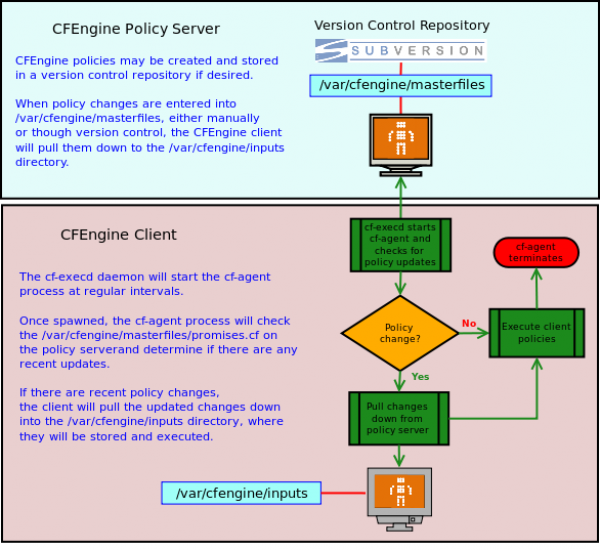
\includegraphics[height=0.8\textheight]{agent-workflow.png}
  \end{center}
\end{frame}

\begin{frame}[fragile]
  \frametitle{Promises}
  ``A promise is the documentation or definition of an intention to
  act or behave in some manner. They are the rules which CFEngine
  clients are responsible for implementing.''\footnote{%
    https://docs.cfengine.com/latest/guide-writing-and-serving-policy.html
  }%

  \begin{semiverbatim}
files:
  \alert<2>{"/tmp/email.[a-z0-9]+"}
  \alert<3>{file_select   => days_old("10"),}
  \alert<4>{delete        => tidy,}
  comment       => "Delete temporary email files";
\end{semiverbatim}

\+
\only<2>{\alert{Target of the promise.} A set of files in this case.}
\only<3>{\alert{Additional criteria for building the promise target.}}
\only<4>{\alert{Action to take.}  In this case, delete all (``tidy'').}
\end{frame}


\begin{frame}
  \frametitle{Promises}
  \begin{center}
    \newcommand\DN{$\blacktriangledown$}

    A promise has three possible outcomes:

    \+
    \begin{tabular}{>{\em}rcc}
    {\bf state is\ldots}    & \multicolumn{2}{c}{\DN state was\ldots \DN} \\
    \multicolumn{1}{c}{\DN} & as promised  & not as such                  \\
    as promised             & {\color{green}\bf kept}
                                           & {\color{violet}\bf repaired}   \\
    not as such             &              & {\color{red}\bf not kept}    \\
    \end{tabular}
  \end{center}
\end{frame}


\begin{frame}[fragile]
  \frametitle{Bundles, I}

  Promises must be grouped into \textbf{bundles}.

  \begin{semiverbatim}
bundle \alert<1>{agent} test \{
  vars:
    "secrets" slist => \{ "/etc/shadow",
                         "/etc/sudoers" \};
  files:
    "$(secrets)"
      create => "false",
      perms  => mog("0400", "root", "root");
\}
  \end{semiverbatim}

%\only<1>{\alert{What CFEngine component should execute this bundle.}
%  More on this later.}
\end{frame}


% \begin{frame}
%   \frametitle{CFEngine 3 components}
%   \begin{center}
%     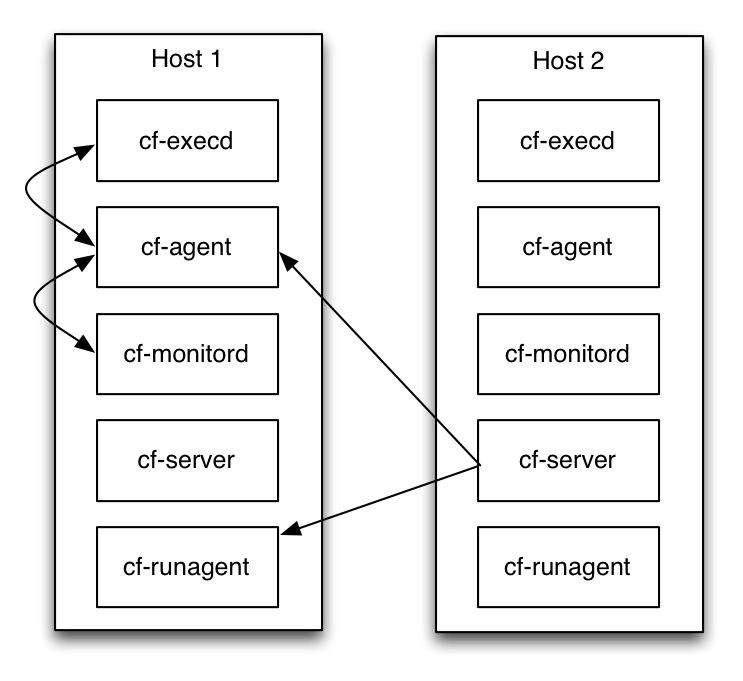
\includegraphics[height=0.8\textheight]{components-overview.png}
%   \end{center}
% \end{frame}

% \begin{frame}[fragile]
%   \frametitle{Bundles, II}

%   Bundles of type \texttt{common} are read by all components.  Other
%   bundles are only read and executed by a single component.  There is
%   rarely any need for non-\texttt{agent} bundles.

%   \begin{semiverbatim}
% bundle common control \{
%   # this is read by \textbf{all} components
%   inputs => \{ "lib/cfengine_stdlib.cf" \};
%   bundlesequence => \{ "test" \};
% \}

% bundle agent test \{
%   # this is only read by `cf-agent`
% \}
%   \end{semiverbatim}
% \end{frame}


\part{(Practice)}

\begin{frame}[fragile]
  \frametitle{Example: keep secret files only readable by root}
  \begin{semiverbatim}
bundle agent keep_secrets \{
  vars:
    "secrets" \alert<1>{slist} => \{ "/etc/shadow",
                         "/etc/sudoers" \};
  files:
    \alert<2>{"$(secrets)"}
      create => "false",
      perms  => mog("0400", "root", "root");
\}
  \end{semiverbatim}

\only<1>{\alert{Define \texttt{secrets} as a \emph{list of strings}}.
  Also available: simple strings, and (fake) integers and floats.}
\only<2>{Since \texttt{secrets} is a \emph{list},
  \alert{this implcitly \emph{loops} over all its values.}}
% \only<3>{\small \texttt{mog()} = mode-owner-group.
%   \alert{It's a standard library \emph{body}.}}
\end{frame}


% \begin{frame}[fragile]
%   \frametitle{Bodies}
%   \begin{columns}
%     \begin{column}{0.75\linewidth}
%       \begin{quote}
%         ``the definition of a promise can grow complicated. Complex
%         promises are best understood by breaking them down into
%         independent, re-usable components. The CFEngine reserved word
%         \texttt{body} is used to encapsulate the details of complex
%         promise attribute values. Bodies can optionally have
%         parameters.''
%       \end{quote}
%     \end{column}
%     \begin{column}{0.5\linewidth}
% \begin{semiverbatim}\small
% body perms secret \{
%  mode   => "0600";
%  owners => \{ "root" \};
%  groups => \{ "root" \};
% \}
% \end{semiverbatim}

% \+
% \begin{semiverbatim}\small
% body perms
%  mog(mode, user,group)
% \{
%  owners=>\{"$(user)"\};
%  groups=>\{"$(group)"\};
%  mode  =>"$(mode)";
% \}
% \end{semiverbatim}
%     \end{column}
%   \end{columns}
%   \begin{references}
%     \url{https://docs.cfengine.com/latest/guide-language-concepts-bodies.html}
%   \end{references}
% \end{frame}


\begin{frame}[fragile]
  \frametitle{Example: edit a file}
\begin{semiverbatim}\small
bundle agent nss_myhostname \{
  files:
      "/etc/nsswitch.conf"
      \alert<1>{edit_line => enable_nss_myhostname;}
\}

bundle \alert<1>{edit_line} enable_nss_myhostname \{
  \alert<2>{replace_patterns:}
      \alert<3>{"(?x) ^hosts:{\textbackslash}s* \alert<4>{(((?!myhostname){\textbackslash}w+{\textbackslash}s+)+)}$"}
      replace_with => value(
        "hosts: $(match.1) myhostname");
\}
\end{semiverbatim}

  \only<1>{Editing is a complex operation, that requires a sequence of
    action. \alert{Therefore, it has a special kind of bundle.}}
  \only<3>{Full \href{http://www.pcre.org/}{PCRE} syntax is supported
    everywhere in CFEngine.}
  \only<4>{\alert{CFEngine will not let you substitute a regexp with a
      string that matches the same regexp!} Need to learn what
    ``negative lookahead assertions'' are\ldots}
  \only<2>{Also available: \texttt{insert\_lines},
    \texttt{delete\_lines}, \texttt{field\_edits}. Which can all be
    combined together.}
\end{frame}


\begin{frame}[fragile]
  \frametitle{Contexts / Classes}
  Contexts\footnote{Previously called ``Classes''}
  are just boolean \textbf{constants}.
  The context ``\texttt{any}'' is CFEngine's alias for ``true''.

  \+
  CFEngine has a concise syntax for ``if'' clauses using contexts:
\begin{semiverbatim}\small
vars:
  \alert<2>{os_centos|os_rhel::
    "rules"     string => "/etc/sysconfig/iptables";}
  os_debian|os_ubuntu::
    "rules"     string => "/etc/iptables/rules.v4";
\end{semiverbatim}

  \only<2>{\alert{
      This part will only be executed when the context
      \texttt{os\_centos} or the context \texttt{os\_rhel} have the
      ``true'' value.}}
\end{frame}


\begin{frame}[fragile]
  \frametitle{Example: deploy template file, I}
\begin{semiverbatim}\small
bundle agent iptables \{
vars:
  os_centos|os_rhel::
    "rules"     string => "/etc/sysconfig/iptables";
  os_debian|os_ubuntu::
    "rules"     string => "/etc/iptables/rules.v4";
  any::
    "www_ports" ilist => \{ "80", "443" \};
files:
  "$(rules)"
  \alert<1>{edit_template  => "iptables.tmpl",}
  \alert<1>{edit_defaults  => empty,}
  perms          => secret,
  create         => "true";
\}
\end{semiverbatim}
  \alert<1>{What template file to use and the initial content of the
    editing buffer.}
\end{frame}

\begin{frame}[fragile]
  \frametitle{Example: deploy template file, II}
  The actual contents of the template file:
\begin{semiverbatim}
# iptables.tmpl
\alert<1>{[% CFEngine www:: %]}
-A INPUT -p tcp --dport \alert<2>{$(www_ports)} -j ACCEPT
[% CFEngine am_policy_hub:: %]
-A INPUT -p tcp --dport 5308 -j ACCEPT
\end{semiverbatim}

  \only<1>{This is the way contexts are applied to templates.  All
    subsequent lines are inserted if and only if context \texttt{www}
    is defined.}
  \only<2>{Since \texttt{www\_ports} is a list, \alert{this implicitly
      loops over all values.}}
\end{frame}


\begin{frame}[fragile]
  \frametitle{Contexts / Classes, II}
  Additionally, contexts can be defined with specific promises, which
  evaluate a boolean expression:
\begin{semiverbatim}\small
classes:
  "os_debian"
  \alert<1>{expression => "debian.!ubuntu";}

  "os_debian6"
  expression => "os_debian\alert<2>&(debian_6|debian_squeeze)";
\end{semiverbatim}

  \only<1>{\alert{Class \texttt{os\_debian} will be defined if class
      \texttt{debian} is defined and class \texttt{ubuntu} is not.}}
\end{frame}


\begin{frame}[fragile]
  \frametitle{Example: install an updated package}
\begin{semiverbatim}\small
bundle agent cve_2014_0160 \{
  vars:
      "to_update" slist => \{"openssl", "libssl1.0.0"\};
    ubuntu_12_04::
      "ok_version" string => "1.0.1-4ubuntu5.12";
    debian_wheezy::
      "ok_version" string => "1.0.1e-2+deb7u5";

  packages:
      "$(to_update)"
      \alert<1>{package_policy  => "update",}
      \alert<2>{package_version => "$(ok_version)",}
      \alert<2>{package_select  => "<=",}
      \alert<3>{package_method  => generic;}
\}
\end{semiverbatim}
  \only<1>{\alert{Action to perform.} Also available:
    \texttt{install}, \texttt{remove}, etc.}
  \only<2>{\alert{When to perform the action.}
    Read: if the installed version is \texttt{<=} of the promised version.}
  \only<3>{\alert{Let CFEngine figure out what package manager to
      use.}  Or you can be explicit and say: \texttt{apt},
    \texttt{yum}, \texttt{rpm}, etc.  }
\end{frame}


\begin{frame}[fragile,fragile]
  \frametitle{Contexts / Classes, III}
  Contexts can be set depending on the outcome of single promises:
\begin{semiverbatim}
files:
  "/etc/locale.gen"
  create    => "false",
  edit_line => uncomment_lines_matching(
                  "(de|en|fr|it)_.+", "#"),
  \alert<1>{classes   => if_repaired("run_localegen");}
\end{semiverbatim}

  \only<1>{\alert{Context \texttt{run\_locale\_gen} will be set if
      this promise is ``repaired''.} One should use it to
    conditionally run the \texttt{locale-gen} command:}
\begin{semiverbatim}
commands:
  os_debian.run_localegen::
    "/usr/sbin/locale-gen";
\end{semiverbatim}
\end{frame}


\begin{frame}[fragile]
  \frametitle{Example: extend CFEngine via modules}
  CFEngine can read back the output of any command and set/unset
  contexts or variables depending on it.
  \begin{columns}
    \begin{column}{0.5\linewidth}
\begin{semiverbatim}\small
bundle local_ctx \{
  commands:
    "cat locals.txt"
    \alert<1>{module => "true";}
\}
\end{semiverbatim}
    \end{column}
    \begin{column}{0.5\linewidth}
\begin{semiverbatim}\small
\alert<4>{# /var/cfengine/locals.txt}
\alert<2>{+pizza_box}
\alert<3>{=location[rack]=10}
\alert<3>{=location[height]=2}
\end{semiverbatim}
    \end{column}
  \end{columns}

  \+
  \only<1>{\alert{Instructs CFEngine to read and parse the command
      output.}}
  \only<2>{\alert{Sets context \texttt{pizza\_box}}}
  \only<3>{\alert{Sets variables \texttt{location[rack]} and
      \texttt{location[height]}}}
  \only<4>{\alert{Any line not starting with \texttt{+}, \texttt{-},
      or \texttt{=} is ignored.}}
\end{frame}


\begin{frame}[fragile]
  \frametitle{Normal ordering}

  \begin{quote}
    ``\alert<1>{Within a bundle, the promise types are executed in a
      round-robin fashion according to so-called normal ordering}
    \emph{[\ldots]}. \alert<2>{The actual sequence continues for up to
      three iterations of the following}, converging towards a final
    state:

    \texttt{meta},
    \texttt{vars},
    \texttt{defaults},
    \texttt{classes},
    \texttt{users},
    \texttt{files},
    \texttt{packages},
    \texttt{guest\_environments},
    \texttt{methods},
    \texttt{processes},
    \texttt{services},
    \texttt{commands},
    \texttt{storage},
    \texttt{databases},
    \texttt{reports}''
  \end{quote}

  \only<1>{Promises in a bundle are \textbf{not} executed in the order
    they are written; rather CFEngine groups them by type and executes
    types in a fixed order.}
  \only<2>{\alert<2>{Note this!} In other words, each promise may be
    re-evaluated up to three times during each bundle run.}

  \begin{references}
    \url{https://docs.cfengine.com/latest/guide-language-concepts-normal-ordering.html}
  \end{references}
\end{frame}


\begin{frame}[fragile]
  \frametitle{Example: send email}
\begin{semiverbatim}\small
bundle agent send_email(to, subj, body) \{
  vars:
      "tmpfile"
      \alert<2>{string => execresult("/bin/mktemp", "noshell");}
  methods:
      "Write body contents into temp file"
      usebundle  => append_to_file("$(tmpfile)",
                                   "$(body)");
  commands:
      "/usr/bin/mail $(to) -s $(subj) <$(tmpfile)";
      "/bin/rm -f '$(tmpfile)'";
\}
\end{semiverbatim}

  \only<2>{\alert{This results in a new file name at each pass.}
    Hence, the bundle never ``converges'' and three emails are sent!}
\end{frame}


\begin{frame}
  \frametitle{What other promise types are there?}
  \begin{description}
    \small
    \item[meta] Information about the bundle, mainly useful for documentation purposes.
    \item[vars] \textbf{Definition of variables}
    \item[defaults] ``Default'' values for bundle parameters
    \item[classes] Definition of additional contexts
    \item[users] Create or delete users in \texttt{/etc/passwd}
    \item[files] \textbf{Create, edit, or audit files}
    \item[packages] \textbf{Install or remove software packages}
    \item[guest\_environments] Control VMs using \emph{libvirt}
    \item[methods] Invoke other bundles
    \item[processes] Stop or signal running processes.
    \item[services] Start or stop system services.
    \item[commands] \textbf{Run arbitrary commands.}
    \item[storage] Mount NFS filesystems.
    \item[databases] Create, alter, or manage DBs and tables on SQL, LDAP, or MS Registry
    \item[reports] Print lines to the log file.
  \end{description}
\end{frame}


\part{(The good, the bad, and the ugly) {\em .reverse(\thinspace)}}
\begin{frame}[fragile]
  \frametitle{The ugly}
  It's (slowly) becoming a programming language, but the syntax is
  verbose and awkward, and is not getting better with time and
  releases:
\begin{semiverbatim}\small
bundle agent sysctl_data \{
vars:
  "parms_vars[net.ipv4.tcp_tw_reuse]" string => "1";
  "parms_test_file" string => "/etc/sysctl";
  "parms_debug" string => "on";
  "parms_mgmt_policy" string => "ensure_present";
methods:
  "test" usebundle => sysctl("sysctl_data.parms_");
\}
\end{semiverbatim}
\end{frame}


\begin{frame}[fragile]
  \frametitle{The bad}

  After more than 6 years, there are still serious bugs in the core
  functionality.

\begin{semiverbatim}\small
$ cat test.cf
{\em [\ldots]}
bundle agent test \{
  vars:
      "variables" slist => variablesmatching(".+");
  reports:
    linux::
      "$(variables)=$($(variables))";
\}

$ time cf-agent -f ./test.cf -b test
{\em [\ldots]}
\textbf{real	43m5.345s}
\end{semiverbatim}

  \+ That, and ``normal ordering.''
\end{frame}


\begin{frame}
  \frametitle{The good}
  Strives to provide \emph{idempotent primitives,} upon which to build
  your own systems administration DSL.

  \+ Can react to changing conditions: facts are not gathered at the
  beginning of the run.

  \+ Can \emph{really} be extended using any language.

  \+ Runs 3'200 (and counting) promises on the top of every hour on
  $O(100)$ hosts in the S${}^3$IT server room, and \emph{keeps all of
    them.} (Really, it can deploy and configure the entire OpenStack
  software suite at a whim.)
\end{frame}


\appendix

\begin{frame}[fragile]
  \frametitle{Further reading}
  \footnotesize
  \begin{description}
    \item[\href{http://shop.oreilly.com/product/0636920022022.do}{Learning CFEngine 3}] The one and only beginners' book.
  \item[\url{https://docs.cfengine.com/docs/3.6/reference-promise-types.html}]
    \emph{The} Reference Manual, you need this every time\ldots
  \item[\url{https://docs.cfengine.com/latest/guide-introduction.html}]
    What the various components are, and how they interact.
  \item[\url{https://docs.cfengine.com/latest/guide-language-concepts.html}]
    Overview of the CFEngine language syntax.
  \item[\url{https://docs.cfengine.com/latest/guide-writing-and-serving-policy-promises-available-in-cfengine.html}]
    Overview of the promise types and best practices for structing a
    CFEngine code base.
  \item[\url{https://docs.cfengine.com/latest/guide-design-center-configure-sketches-community.html}]
    Desgin Center / Sketches: how to re-use CFEngine code packaged and shared by others.
  \end{description}
\end{frame}


\begin{frame}
  \frametitle{%
    {\color{blue} CFEngine}
    {\color{red} Puppet}
    {\color{yellow} Salt Stack}
    {\color{green} Ansible}
    {\color{violet} Chef}
  }%
  \begin{center}
    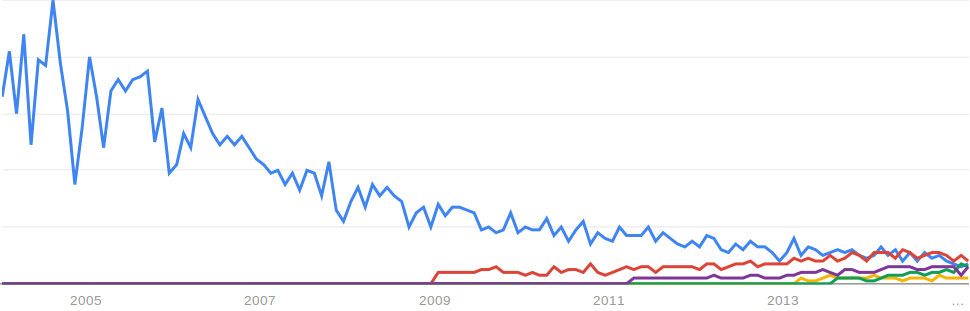
\includegraphics[width=1.0\linewidth]{google-trends-since-2004.png}

    {\footnotesize\em Google trends:
      2004--today ($\blacktriangle$),
      2009--today ($\blacktriangledown$)}

    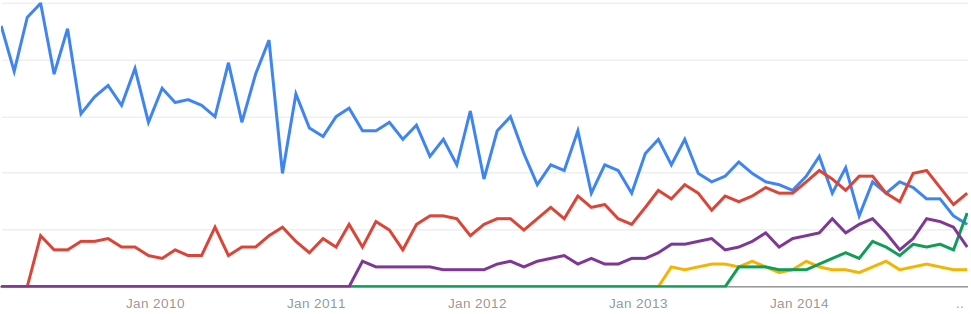
\includegraphics[width=1.0\linewidth]{google-trends-since-2009.png}
  \end{center}
\end{frame}

\end{document}

%%% Local Variables:
%%% mode: latex
%%% TeX-master: t
%%% End:
